\documentclass[
a4paper,   
headsepline, 
fleqn,     
11pt
]{scrartcl}

%%% ngerman: language set to new-german
\usepackage{ngerman}
\usepackage[utf8]{inputenc}
\usepackage[T1]{fontenc}
\usepackage{ae,aecompl}

%%% Graphic stuff
\usepackage{graphicx}
\usepackage{geometry}
\geometry{verbose,a4paper,tmargin=25mm,bmargin=25mm,lmargin=15mm,rmargin=20mm}
\usepackage{amsmath,amssymb,amstext}
\usepackage{units}
\usepackage{scrpage2}

%%% comments, ...
\usepackage{verbatim}

\setlength{\parindent}{0em} 

\renewcommand*\thesection{\Alph{section}}

\newcommand{\mygraphics}[3]{
  \begin{center}
    \includegraphics[width=#1, keepaspectratio=true]{#2} \\
    \textbf{#3}
  \end{center}
}

%%%      footer - middle: page number
\pagestyle{scrheadings}

%%% heading - left
 \ihead[]{Marco Sohm, Kevin Wallis}

%%% heading - right
 \ohead[]{Aufgabe 3}

\begin{document}

 \pagenumbering{roman} %% small roman page numbers
 \pagenumbering{arabic} 

\section{Modellieren des Systems in AnyLogic}
Das System wurde wie gewünscht in AnyLogic modelliert. Die vorgegebenen Werte wurden vollständig in das Model übernommen. In der nachstehenden Liste sind die wesentlichen Werte aufgereiht. 

\begin{itemize}
	\item Terminals $=10$
	\item Denkzeit im Mittel $=25s$
	\item Maximale Rechenzeit $=0.1s$
	\item Overhead swapping $=0.015s$
	\item Mittlere CPU Zeit $=0.8s$
\end{itemize}

Die Modellierung ist sehr objektorientiert und kann daher leicht erweitert werden. Die mittlere Denkzeit und die mittlere Zeit an CPU Bedarf kann für jedes Terminal einzeln eingestellt werden, ist jedoch aufgrund der Verwendung von Replicated Object bei jedem Terminal gleich. In Grafik \ref{fig:SimulationA} ist ersichtlich, dass der Steady State ungefähr bei $40.000s$ eintritt.

\textbf{Erklärung des Ergebnisses:} Es ist zu erkennen, dass zu Beginn eine 

\section{Definieren der Zielfunktion}
\label{sec:DefinitionTargetFunction}
Die Zielfunktion wurde wie folgt definiert: \\
\textit{Die mittlere reine Wartezeit des Terminalbenutzers, die als Wartezeit zwischen Absenden und Empfangen eines Jobs minus der benötigten CPU Rechenzeit definiert ist, und davon den über alle Terminals gemittelten Wert.}

Es wurde ein Parameterexperiment durchgeführt um die Abhängigkeit die Zielfunktion von der Zeitscheibendauer aufzuzeigen, dieses ist in Grafik \ref{fig:ParametervariationB-02} zu sehen.

Weitere Parametervariation die durchgeführt wurden sind im Folgenden aufgelistet.

\begin{itemize}
	\item XXX
	\item XXX
\end{itemize}

\section{Optimieren der Zeitscheibendauer}
Der Defaultwert der Zeitscheibendauer wurden mithilfe von Optimierungsexperimenten ermittelt. In Abbildung \ref{fig:OptimizationC} ist das Ergebnis dargestellt, hierbei ist ersichtlich, dass sich das Zeitscheibendauer - Optimum bei dem Wert $0.106s$ befindet. Auch wurde festgestellt, dass dieser Wert mit der Simulation aus \ref{sec:DefinitionTargetFunction} übereinstimmt und mit Grafik \ref{fig:ParametervariationB} verglichen werden kann.

\section{Äquivalenz zu Round Robin}
Diese Frage muss, wie in der Lehrveranstaltung besprochen, nicht bearbeitet werden.

\newpage

\subsection*{Anhang}
Im Folgenden sind die unterschiedlichen Simulationsergebnisse der CPU - Aufgabe zu finden.

\begin{figure}[h]
  \centering
  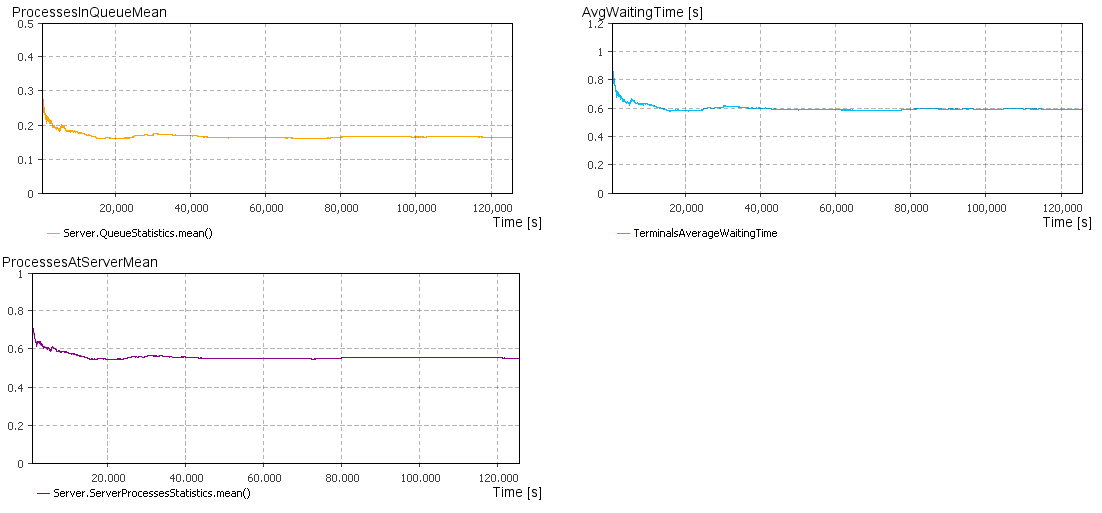
\includegraphics[width=1\textwidth]{./images/Simulation_SteadyState}
  \caption{Simulation des CPU Models, mit Steady State}
  \label{fig:SimulationA}
\end{figure}

\begin{figure}[h]
  \centering
  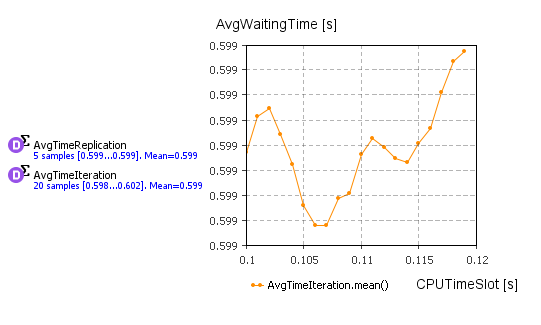
\includegraphics[width=1\textwidth]{./images/ParameterVariationCPUTimeSlot}
  \caption{Parametervariation der Zeitscheibendauer}
  \label{fig:ParametervariationB}
\end{figure}

\begin{figure}[h]
  \centering
  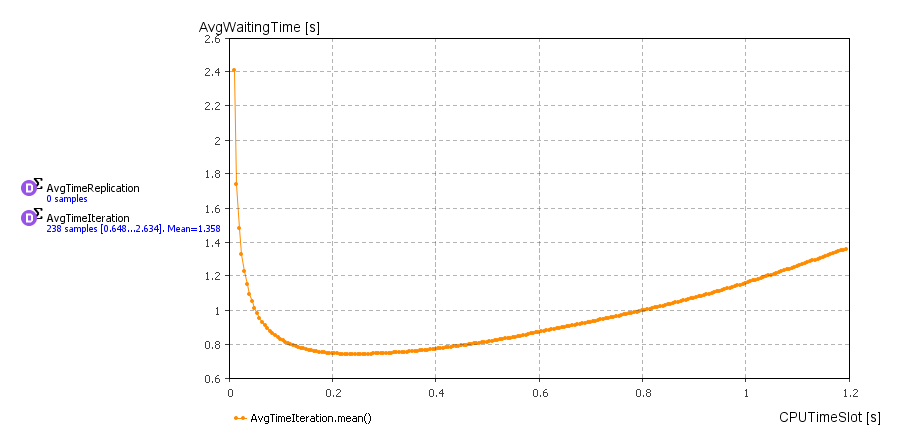
\includegraphics[width=1\textwidth]{./images/ParameterVariationCPUTimeSlot_StopTime4000}
  \caption{Parametervariation der Zeitscheibendauer}
  \label{fig:ParametervariationB-02}
\end{figure}

\begin{figure}[h]
  \centering
  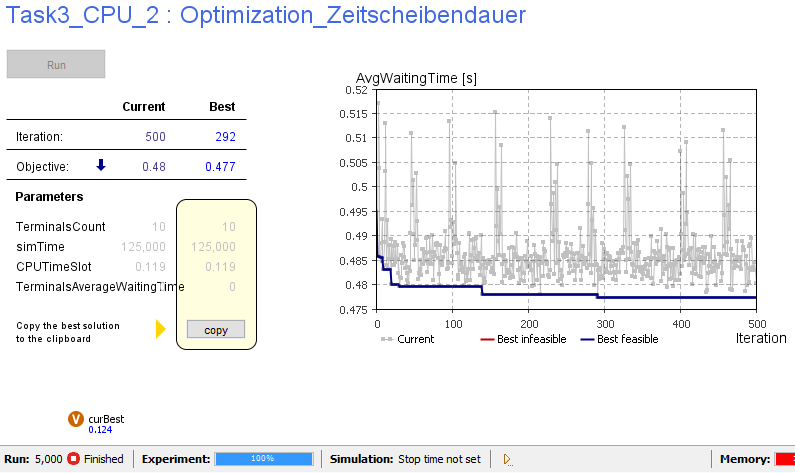
\includegraphics[width=1\textwidth]{./images/Optimization}
  \caption{Optimierung der Zeitscheibendauer}
  \label{fig:OptimizationC}
\end{figure}

\appendix  
\bibliographystyle{plain}
\bibliography{projekt.bib}

\end{document}